\documentclass[11pt,a4paper]{article}

% French
\usepackage[utf8x]{inputenc}
\usepackage[frenchb]{babel}
\usepackage[T1]{fontenc}
\usepackage{lmodern}
\usepackage{ifthen}

% Color
% cfr http://en.wikibooks.org/wiki/LaTeX/Colors
\usepackage{color}
\usepackage[usenames,dvipsnames,svgnames,table]{xcolor}
\definecolor{dkgreen}{rgb}{0.25,0.7,0.35}
\definecolor{dkred}{rgb}{0.7,0,0}

% Floats and referencing
\newcommand{\sectionref}[1]{section~\ref{sec:#1}}
\newcommand{\annexeref}[1]{annexe~\ref{ann:#1}}
\newcommand{\figuref}[1]{figure~\ref{fig:#1}}
\newcommand{\tabref}[1]{table~\ref{tab:#1}}
\usepackage{xparse}
\NewDocumentEnvironment{myfig}{mm}
{\begin{figure}[!ht]\centering}
{\caption{#2}\label{fig:#1}\end{figure}}

% Listing
\usepackage{listings}
\lstset{
  numbers=left,
  numberstyle=\tiny\color{gray},
  basicstyle=\rm\small\ttfamily,
  keywordstyle=\bfseries\color{dkred},
  frame=single,
  commentstyle=\color{gray}=small,
  stringstyle=\color{dkgreen},
  %backgroundcolor=\color{gray!10},
  %tabsize=2,
  rulecolor=\color{black!30},
  %title=\lstname,
  breaklines=true,
  framextopmargin=2pt,
  framexbottommargin=2pt,
  extendedchars=true,
  inputencoding=utf8x
}

\newcommand{\matlab}{\textsc{Matlab}}
\newcommand{\octave}{\textsc{GNU/Octave}}
\newcommand{\qtoctave}{\textsc{QtOctave}}
\newcommand{\oz}{\textsc{Oz}}
\newcommand{\java}{\textsc{Java}}
\newcommand{\clang}{\textsc{C}}
\newcommand{\keyword}{mot clef}

% Math symbols
\usepackage{amsmath}
\usepackage{amssymb}
\usepackage{amsthm}
\DeclareMathOperator*{\argmin}{arg\,min}
\DeclareMathOperator*{\argmax}{arg\,max}

% Sets
\newcommand{\Z}{\mathbb{Z}}
\newcommand{\R}{\mathbb{R}}
\newcommand{\Rn}{\R^n}
\newcommand{\Rnn}{\R^{n \times n}}
\newcommand{\C}{\mathbb{C}}
\newcommand{\K}{\mathbb{K}}
\newcommand{\Kn}{\K^n}
\newcommand{\Knn}{\K^{n \times n}}

% Chemistry
\newcommand{\std}{\ensuremath{^{\circ}}}
\newcommand\ph{\ensuremath{\mathrm{pH}}}

% Theorem and definitions
\theoremstyle{definition}
\newtheorem{mydef}{Définition}
\newtheorem{mynota}[mydef]{Notation}
\newtheorem{myprop}[mydef]{Propriétés}
\newtheorem{myrem}[mydef]{Remarque}
\newtheorem{myform}[mydef]{Formules}
\newtheorem{mycorr}[mydef]{Corrolaire}
\newtheorem{mytheo}[mydef]{Théorème}
\newtheorem{mylem}[mydef]{Lemme}
\newtheorem{myexem}[mydef]{Exemple}
\newtheorem{myineg}[mydef]{Inégalité}

% Unit vectors
\usepackage{esint}
\usepackage{esvect}
\newcommand{\kmath}{k}
\newcommand{\xunit}{\hat{\imath}}
\newcommand{\yunit}{\hat{\jmath}}
\newcommand{\zunit}{\hat{\kmath}}

% rot & div & grad & lap
\DeclareMathOperator{\newdiv}{div}
\newcommand{\divn}[1]{\nabla \cdot #1}
\newcommand{\rotn}[1]{\nabla \times #1}
\newcommand{\grad}[1]{\nabla #1}
\newcommand{\gradn}[1]{\nabla #1}
\newcommand{\lap}[1]{\nabla^2 #1}


% Elec
\newcommand{\B}{\vec B}
\newcommand{\E}{\vec E}
\newcommand{\EMF}{\mathcal{E}}
\newcommand{\perm}{\varepsilon} % permittivity

\newcommand{\bigoh}{\mathcal{O}}
\newcommand\eqdef{\triangleq}

\DeclareMathOperator{\newdiff}{d} % use \dif instead
\newcommand{\dif}{\newdiff\!}
\newcommand{\fpart}[2]{\frac{\partial #1}{\partial #2}}
\newcommand{\ffpart}[2]{\frac{\partial^2 #1}{\partial #2^2}}
\newcommand{\fdpart}[3]{\frac{\partial^2 #1}{\partial #2\partial #3}}
\newcommand{\fdif}[2]{\frac{\dif #1}{\dif #2}}
\newcommand{\ffdif}[2]{\frac{\dif^2 #1}{\dif #2^2}}
\newcommand{\constant}{\ensuremath{\mathrm{cst}}}

% Numbers and units
\usepackage[squaren, Gray]{SIunits}
\usepackage{sistyle}
\usepackage[autolanguage]{numprint}
%\usepackage{numprint}
\newcommand\si[2]{\numprint[#2]{#1}}
\newcommand\np[1]{\numprint{#1}}

\newcommand\strong[1]{\textbf{#1}}
\newcommand{\annexe}{\part{Annexes}\appendix}

% Bibliography
\newcommand{\biblio}{\bibliographystyle{plain}\bibliography{biblio}}

\usepackage{fullpage}
% le `[e ]' rend le premier argument (#1) optionnel
% avec comme valeur par défaut `e `
\newcommand{\hypertitle}[7][e ]{
\usepackage{hyperref}
{\renewcommand{\and}{\unskip, }
\hypersetup{pdfauthor={#6},
            pdftitle={Synth\`ese d#1#2 Q#3 - L#4#5},
            pdfsubject={#2}}
}

\title{Synth\`ese d#1#2 Q#3 - L#4#5}
\author{#6}

\begin{document}

\ifthenelse{\isundefined{\skiptitlepage}}{
\begin{titlepage}
\maketitle

 \paragraph{Informations importantes}
   Ce document est grandement inspiré de l'excellent cours
   donné par #7 à l'EPL (École Polytechnique de Louvain),
   faculté de l'UCL (Université Catholique de Louvain).
   Il est écrit par les auteurs susnommés avec l'aide de tous
   les autres étudiants, la vôtre est donc la bienvenue.
   Il y a toujours moyen de l'améliorer, surtout si le cours
   change car la synthèse doit alors être modifiée en conséquence.
   On peut retrouver le code source à l'adresse suivante
   \begin{center}
     \url{https://github.com/Gp2mv3/Syntheses}.
   \end{center}
   On y trouve aussi le contenu du \texttt{README} qui contient de plus
   amples informations, vous êtes invité à le lire.

   Il y est indiqué que les questions, signalements d'erreurs,
   suggestions d'améliorations ou quelque discussion que ce soit
   relative au projet
   sont à spécifier de préférence à l'adresse suivante
   \begin{center}
     \url{https://github.com/Gp2mv3/Syntheses/issues}.
   \end{center}
   Ça permet à tout le monde de les voir, les commenter et agir
   en conséquence.
   Vous êtes d'ailleurs invité à participer aux discussions.

   Vous trouverez aussi des informations dans le wiki
   \begin{center}
     \url{https://github.com/Gp2mv3/Syntheses/wiki}.
   \end{center}
   comme le statut des synthèses pour chaque cours
   \begin{center}
     \url{https://github.com/Gp2mv3/Syntheses/wiki/Status}.
   \end{center}
   vous pouvez d'ailleurs remarquer qu'il en manque encore beaucoup,
   votre aide est la bienvenue.

   Pour contribuer au bug tracker et au wiki, il vous suffira de
   créer un compte sur Github.
   Pour interagir avec le code des synthèses,
   il vous faudra installer \LaTeX.
   Pour interagir directement avec le code sur Github,
   vous devez utiliser \texttt{git}.
   Si cela pose problème,
   nous sommes évidemment ouverts à des contributeurs envoyant leurs
   changements par mail ou n'importe quel autre moyen.
\end{titlepage}
}{}

\ifthenelse{\isundefined{\skiptableofcontents}}{
\tableofcontents
}{}
}


\usepackage{graphicx}
\usepackage{verbatim}

\lstset{language=SQL}

\hypertitle{Conception orientée objet et gestion de bases de données}
{4}{SINF}{1225}{Benjamin de Wergifosse}{Benjamin de Wergifosse}

\section{Gérer une base de données avec le langage SQL}
Une base de données permet de stocker des informations de manières structurées
et facilement accessible.
Les données y sont organisées en tables selon un thème,
une \textbf{collection d'entités} (ex. Clients, Réservations,...).
Il faut cependant veiller à créer ces tables de manières intelligentes:
il faut
\begin{itemize}
  \item éviter les données redondantes
    (que l'on peut trouver grâce à d'autres),
  \item veiller à ce qu'on puisse faire le lien entre les différentes
    tables grâce à des références (ID),
  \item éviter les redondances au sein d'une même table
    ($\Rightarrow$ on split la table).
\end{itemize}

Dans une table,
si une colonne est constituée de valeurs uniques,
on dit qu'elle est un \textbf{identifiant} de la table,
elle constitue une \textbf{clé primaire}.
Si une colonne contient des informations (un ID par exemple) qui permettent
de récupérer des informations associées dans une autre table,
on nomme la colonne de \textbf{clé étrangère}.

Une base de données se gère grâce au langage SQL
qui possède une syntaxe particulière.
Nous allons voir les principales requêtes permettant d'accéder aux données,
de les modifier et d'en ajouter.
D'autres parts, un logiciel,
que l'on nomme \textbf{système de gestion de bases de données},
permet la gestion sur disque des tables.
Il assure la sécurité, la confidentialité,
l'archivage et la restauration des informations.
Les requêtes SQL sont envoyées au programme qui les comprends et
va chercher sur le disque les informations relatives aux requêtes.
On utilisera SQLite,
un SGBD léger et efficace utilisé par les applications Android et iOS.

\subsection{Les requêtes de base}
\begin{lstlisting}
SELECT - extracts data from a database
UPDATE - updates data in a database
DELETE - deletes data from a database
INSERT INTO - inserts new data into a database

CREATE DATABASE - creates a new database
ALTER DATABASE - modifies a database
CREATE TABLE - creates a new table
ALTER TABLE - modifies a table
DROP TABLE - deletes a table
CREATE INDEX - creates an index (search key)
DROP INDEX - deletes an index
\end{lstlisting}

\subsection{SELECT statement}
\begin{lstlisting}
SELECT LastName,FirstName FROM Persons
SELECT * FROM Persons
SELECT DISTINCT City FROM Persons
\end{lstlisting}

\subsection{WHERE clause}
\begin{lstlisting}
SELECT column_name(s) FROM table_name WHERE column_name operator value

With the WHERE clause, the following operators can be used:
Operator  Description
=         Equal
<>        Not equal
>         Greater than
<         Less than
>=        Greater than or equal
<=        Less than or equal
BETWEEN   Between an inclusive range
LIKE      Search for a pattern
IN        To specify multiple possible values for a column
/* Note: In some versions of SQL the <> operator
 * may be written as !=
 */
\end{lstlisting}

\subsection{AND \& OR operators}
\begin{lstlisting}
SELECT * FROM Persons WHERE LastName='Svendson' AND (FirstName='Tove' OR FirstName='Ola')
\end{lstlisting}

\subsection{ORDER BY keyword}
\begin{lstlisting}
SELECT * FROM Persons ORDER BY LastName DESC
\end{lstlisting}

\subsection{INSERT INTO statement}
\begin{lstlisting}
INSERT INTO table_name VALUES (value1, value2, value3,...)
INSERT INTO table_name (column1, column2, column3,...) VALUES (value1, value2, value3,...)
\end{lstlisting}

\subsection{UPDATE statement}
\begin{lstlisting}
UPDATE table_name SET column1=value, column2=value2,... WHERE some_column=some_value AND some_column=some_value AND ...
\end{lstlisting}

\subsection{DELETE statement}
\begin{lstlisting}
DELETE FROM table_name WHERE some_column=some_value AND some_column=some_value AND ...
\end{lstlisting}

\subsection{Examples of queries}
\begin{lstlisting}
select NCOM
from COMMANDE M, CLIENT C
where M.NCLI = C.NCLI
and C.LOCALITE = 'Toulouse';

select NCOM
from COMMANDE
where NCLI in
(select NCLI
from CLIENT where LOCALITE = 'Toulouse');
\end{lstlisting}

\subsection{Création d'une table}
\begin{lstlisting}
create table CLIENT (
  NCLI char(10) not null primary key,
  NOM char(32) not null unique,
  ADRESSE char(60) not null,
  LOCALITE char(30) not null,
  CAT char(2),
  COMPTE decimal(9,2) not null );
\end{lstlisting}

\subsection{Création d'une table relationnelle}
\begin{lstlisting}
create table COMMANDE (
  NCOM char(12) not null,
  NCLI char(10) not null,
  DATECOM date not null,
  primary key (NCOM),
  foreign key (NCLI) references CLIENT);
/* ou de maniere equivalente */
create table COMMANDE (
  NCOM char(12) not null primary key,
  NCLI char(10) not null references CLIENT,
  DATECOM date not null);
\end{lstlisting}

\subsection{Modification et suppression d'une table NON RELATIONNELLE}
\begin{lstlisting}
alter table PRODUIT add column POIDS smallint;

drop table CLIENT;
\end{lstlisting}

\subsection{Une sélection simple dans une table}
\begin{lstlisting}
select distinct LOCALITE
from CLIENT
where CAT = 'C1';

select NCLI
from CLIENT
where CAT is null; /* ATTENTION PAS CAT = null */

select NCLI
from CLIENT
where CAT is not null;
\end{lstlisting}

\subsection{Une sélection avec condition(s)}
\begin{lstlisting}
select NCLI
from CLIENT
where CAT in ('C1','C2','C3');

select NCLI
from CLIENT
where LOCALITE not in ('Toulouse','Breda');

select NCLI
from CLIENT
where COMPTE between 1000 and 4000;

select NCLI
from CLIENT
where CAT like 'B_';
/* exemple : 'B1' 'Bd' 'B '
 * mais pas : 'xB' 'B' 'B12'
 */

select NPRO
from PRODUIT
where LIBELLE like '%SAPIN%';
/* exemple : 'PL. SAPIN 200x20x2' */
'Boite en SAPIN'
'SAPIN VERNI'

select LIBELLE
from PRODUIT
where LIBELLE like '%produit avec un !_%'
/* on utilise un caractere d echappement */
escape '!';
\end{lstlisting}

\subsection{Une sélection avec calcul}
\begin{lstlisting}
select 'TVA de ', NPRO, ' = ', 0.21*PRIX*QSTOCK
from PRODUIT
where QSTOCK > 500;
\end{lstlisting}

\subsection{Une sélection avec alias}
\begin{lstlisting}
select NPRO as Produit, 0.21*PRIX*QSTOCK as Valeur_TVA
from PRODUIT
where QSTOCK > 500;
\end{lstlisting}

\subsection{Les conditions de jointures}
\begin{lstlisting}
select NCOM,
DATECOM,
CLIENT.NCLI, /* .NCLI obligatoire car ambiguite sinon */
NOM,
LOCALITE
from COMMANDE, CLIENT
where COMMANDE.NCLI = CLIENT.NCLI;
/* NCLI est une colonne commune dans les deux tables */
\end{lstlisting}

\subsection{Deux requêtes équivalentes avec jointures}
\begin{lstlisting}
select NCOM,DATECOM
from COMMANDE
where NCLI in (select NCLI
from CLIENT
where LOCALITE = 'Poitiers');

select NCOM,DATECOM
from COMMANDE, CLIENT
where COMMANDE.NCLI = CLIENT.NCLI
and LOCALITE = 'Poitiers';
\end{lstlisting}

\subsection{Insertion}
\begin{lstlisting}
insert into DETAIL
values ('30185','PA45',12);

insert into CLIENT (NCLI,NOM,ADRESSE,COMPTE,LOCALITE)
values ('C402','BERNIER','avenue de France, 28',-2500,'Lausanne');

insert into CLIENT_TOULOUSE
select NCLI, NOM, ADRESSE
from CLIENT
where LOCALITE = 'Toulouse';
\end{lstlisting}

\subsection{Suppression de ligne}
\begin{lstlisting}
delete from CLIENT
where NCLI = 'K111';

delete from DETAIL
where NPRO in (select NPRO
from PRODUIT
where QSTOCK <= 0);

delete from CLIENT
where CAT is null;
\end{lstlisting}

\subsection{Update de ligne}
\begin{lstlisting}
update CLIENT
set ADRESSE = '29, av. de la Magne',
LOCALITE = 'Niort'
where NCLI = 'F011';

update PRODUIT
set PRIX = PRIX * 1.05
where LIBELLE like '%SAPIN%';
\end{lstlisting}

\section{Modélisation de données ORM et mapping relationnel}
Dans le processus de développement d'une application orientée objet,
il est important de bien penser son application avant de se
pencher sur l'implémentation de son code source.
Ainsi diverses étapes d'analyse du problème sont requises.
La modélisation de données selon l'approche
ORM (Object-Role Modeling) est en la première.

Dans un premier temps,
il est important de définir \textbf{l'univers de discours} (UoD).
Celui-ci, en une phrase, définit le domaine de l'application.

\subsection{Le modèle relationnel et les relations n-aires}
On cherche à définir les relations qui existent.
Ces relations définiront les tables SQL qui seront créées.
À une relation correspondra une table.
Le \textbf{schéma de la relation} reprend les noms des colonnes de
la table qui lui correspondra.
Par exemple, on pourrait imaginer le schéma de la relation Client suivant:
\begin{lstlisting}
CLIENT(ID, SORTE, NOM, PRENOM, ADRESSE)
\end{lstlisting}
Dans le modèle relationnelle, on n'utilise pas la notation positionnelle.
Dès lors, un mutliplet Client sera toujours
un ensemble de couple \lstinline$(TITRE, valeur)$.
On pourrait imaginer la \textbf{relation} basée sur
le schéma ci-dessus comme étant l'ensemble de multiplets suivant:
\begin{lstlisting}
{
  {(ID,459), (SORTE,externe), (NOM,Horner), (PRENOM,Yvette), (ADRESSE,"7, impasse des capucines, Wavre")},
  {(ID,3124), (SORTE,interne), (NOM,Dupont), (PRENOM,Jules), (ADRESSE,"3, rue des combattants, La Hulpe")},
  ...,
  {(ID,6789), (SORTE,externe), (NOM,Gave), (PRENOM,Jean), (ADRESSE,"32, avenue des allies, Tournai")},
  {(ID,6947), (SORTE,interne), (NOM,Durant), (PRENOM,Alfred), (ADRESSE,"17, allee des saules, Plancenoit")}
}
\end{lstlisting}
Le transfert de cette relation vers une table est immédiat.
La base de données est donc un ensemble de table basées
sur un ensemble de relations $n$-aires.
La \textbf{schéma de la base de données} n'est
autre que l'ensemble des schémas des différentes relations.

\subsection{L'Object-Role Modeling}
Fortement basé sur le modèle relationnel simple présenté ci-dessus,
l'ORM en est une amélioration qui permet d'éviter les redondances,
qui est plus conforme au monde réel et plus intuitif et facile à comprendre.
Cette approche tient compte du fait qu'une base de données
peut être vue comme un ensemble de \textbf{faits} (les données)
et de \textbf{règles} (liens entre les faits) s'articulant autour
d'un \textbf{univers de discours}.
Ainsi, 3 étapes permettent la modélisation ORM.

\subsubsection{Les faits élémentaires}
Premièrement,
il faut, en se basant sur des exemples de données,
établir une liste de \textbf{faits élémentaires}.
Un fait élémentaire est une assertion simple et atomique
sur l'univers de discours.
Un fait élémentaire fait intervenir des \textbf{objets} et leur \textbf{rôle}.
Il y a deux types d'objets:
les VALEURS et les entités (= ensemble TYPE-MODE-VALEUR).
Exemples:
\begin{itemize}
  \item Client-nom-``UCL''
  \item Facture-numéro-0254968065768
  \item Montant-euro-275
\end{itemize}

Selon qu'un fait élémentaire fait intervenir plus ou moins d'objets
on dira qu'elle est \textbf{unaire} (1),
\textbf{binaire} (2) ou \textbf{n-aire} (n).
Voici quelques exemples de faits élémentaires :
\begin{itemize}
  \item Destination-numéro-0475151230 \emph{est gratuite}
  \item Opérateur-nom-``Proximus'' \emph{a} Préfixe-numéro-0478
  \item Communication-numéro-11 \emph{a} Durée-minutes-``1:38''
  \item Facture-numéro-0648979136879 \emph{coûte} Montant-euro-289
  \item Etudiant-noma-54511100 \emph{a obtenu} Cote-chiffre-18
    \emph{pour} Cours-code-``LSINF1125''
\end{itemize}
Il est à noter qu'un fait élémentaire ne peut pas être divisé et
qu'il n'utilise aucun connecteurs logiques (et, ou, non, si).

\subsubsection{Dessiner les types de faits + population}
Le but de cette étape est de créer un \textbf{schéma conceptuel}
(voir figure~\ref{schema_conceptuel}).
Pour cela il faut identifié les TYPES d'objets, leur MODE (type de valeur)
et la relation n-aire s'y rapportant.
L'exemple n'illustre que des relations binaires mais l'extension
à la relation ternaire est immédiate
(ajout d'une boite sur la ligne de relation).
\begin{figure}[h]
  \centering
  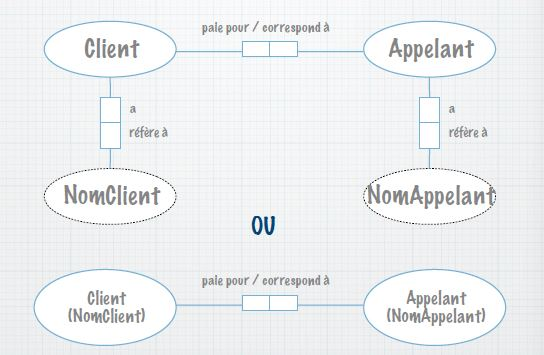
\includegraphics[scale=0.7]{schema_conceptuel.jpg}
  \caption{Exemple d'un schéma conceptuel}
  \label{schema_conceptuel}
\end{figure}
Une fois le schéma créé,
il faut lui ajouter une population exemple pour
s'assurer de l'exactitude de celui-ci.

\subsubsection{Les contraintes}
Le schéma est encore loin d'être terminé,
il faut maintenant lui ajouter les \textbf{contraintes d'unicité}
(voir figure~\ref{contraintes}).
Ces contraintes permettent de déterminer si un valeur peut se retrouver
une ou plusieurs fois dans une même colonne.
Une bonne population exemple facilite le choix des contraintes.
L'exemple donné illustre les contraintes pour la relation binaire mais
l'extension pour le cas ternaire est immédiate.
Dans ce cas,
il est évident qu'il n'y aura jamais de contrainte ``simple''
auquel cas on pourrait diviser la relation en deux autres binaires.
\begin{figure}[h]
  \centering
  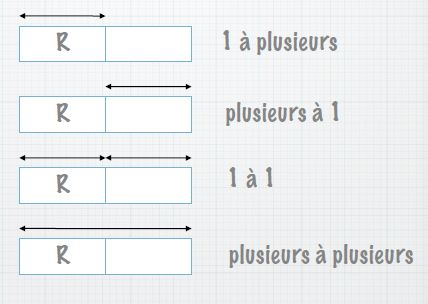
\includegraphics[scale=0.8]{contraintes.jpg}
  \caption{Contraintes possibles pour une relation binaire}
  \label{contraintes}
\end{figure}

Il faut également ajouter les contraintes de \textbf{rôles obligatoires}.
En effet il se peut que l'on veille stipuler que la relation
liant deux objets doit être obligatoire.
Pour ce faire, on place un point sur la ligne de relation.

Une autre contrainte à ajouter sur le schéma conceptuel est celle
d'\textbf{unicité externe}.
En effet, il se peut qu'un objet ayant plusieurs relations soit déterminé
de manière uniquement par la combinaison de plusieurs objets avec lesquels
il est en relation.
Par exemple un fichier qui serait en relation avec un dossier et un nom de
fichier est déterminé
de manière unique par la combinaison dossier-nom\_de\_fichier.

La dernière contrainte possible est la \textbf{contrainte de sous-ensemble}.
Cette contrainte stipule qu'une relation ne peut exister que
si une autre (qui n'est donc pas obligatoire) est satisfaite.

\begin{figure}[h]
  \centering
  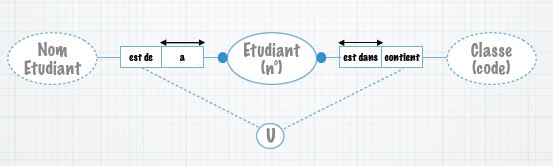
\includegraphics[scale=0.8]{schema_conceptuel_complet}
  \caption{Exemple complet d'un schéma conceptuel}
  \label{schema_conceptuel_complet}
\end{figure}

La figure~\ref{schema_conceptuel_complet} montre comment dessiner ces
contraintes sur le schéma conceptuel.
La contrainte de sous-ensemble, plus rare,
se dessine comme une flèche en pointillé de boite à boite obligatoire
(un peu comme l'unicité externe).


\subsection{Schéma relationnel}
Après avoir transformer les relations n-aires du modèle relationnel
en schéma conceptuel ORM,
il est maintenant temps de transformer le schéma conceptuel
ORM et \textbf{schéma relationnel}.

Le principe consiste à choisir un objet clé du schéma conceptuel
et de le transcrire sous forme de tableau.
Dans ce tableau doit ce retrouvé toutes les contraintes du schéma conceptuel.
Ainsi,
\begin{itemize}
  \item la contrainte d'unicité donnera lieu à une clé primaire et sera
    souligné une fois si il n'y a pas d'autres clés secondaires
    (deux fois sinon).
  \item la contrainte d'unicité externe donnera lieu à une clé secondaire et
    sera souligné une fois
    (avec des flèches si les entités ne sont pas voisines)
  \item le rôle obligatoire s'exprimera par le fait qu'on encadrera les entités
    optionnelles; les autres étant donc obligatoires.
  \item la contrainte de sous-ensemble se manifestera par une flèche reliant
    les deux clés primaires des tableaux différents
    (si toutefois les données sont dans deux tableaux différents)
\end{itemize}

La figure~\ref{schema_relationnel} illustre un exemple de schéma relationnel
avec les différentes contraintes représentées.
\begin{figure}[h]
  \centering
  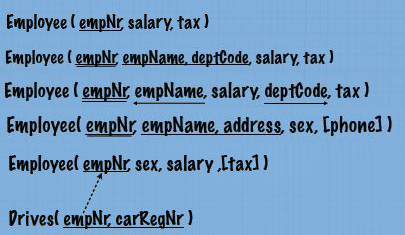
\includegraphics[scale=0.9]{schema_relationnel.jpg}
  \caption{Exemple schéma relationnel}
  \label{schema_relationnel}
\end{figure}

Dans un tableau, une clé primaire ne peut jamais être nulle,
une clé primaire est donc une colonne obligatoire.
Il s'agit de la \textbf{règle d'intégrité des entités}.
D'autres parts, lors d'une contrainte de sous-ensemble,
la flèche venant de la clé étrangère doit pointer vers une clé primaire.
Il s'agit de la \textbf{règle d'intégrité référentielle}.

La figure~\ref{conceptuel_to_relationnel} illustre un exemple un peu plus
élaboré du passage d'un schéma conceptuel vers un schéma relationnel.
\begin{figure}[ht]
  \centering
  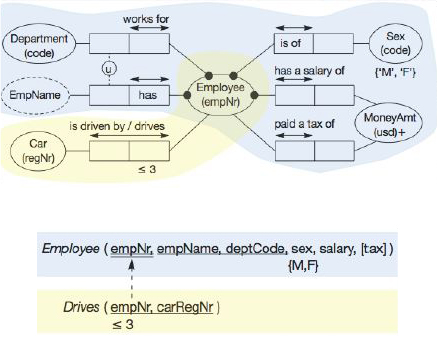
\includegraphics[scale=1]{conceptuel_to_relationnel.jpg}
  \caption{Exemple du passage d'un schéma conceptuel vers un schéma relationnel}
  \label{conceptuel_to_relationnel}
\end{figure}


\subsection{Le Relational Mapping}
Cette dernière étape permet, à partir du schéma relationnel,
de construire la base de données SQL.
La règle est relativement simple, deux règles sont à respecter:
\begin{enumerate}
  \item Les types de faits avec contraintes d'unicité composées
    sont mis dans des tableaux séparés.
  \item Tous les types de faits avec des rôles fonctionnels (unicité simple)
    liés à un même type d'objet sont regroupé dans un même tableau
    avec comme clé l'identifiant de ce type d'objet.
\end{enumerate}

\section{Processus de développement}
Dans la section précédente, nous avons vu comment modéliser,
de manière efficace, les données qui seront utilisées par l'application.
Cette modélisation par l'approche ORM nous a permis d'obtenir une solide
base de données SQL.
À présent, il est temps de se pencher sur la question de l'implémentation.
Comment va-t-on implémenter notre application, que doit-elle pouvoir faire,...
Il est important de suivre un \textbf{processus de développement}
rigoureux qui nous permettra d'implémenter une bonne application.
Observons différents processus possibles.

\begin{figure}[h]
  \centering
  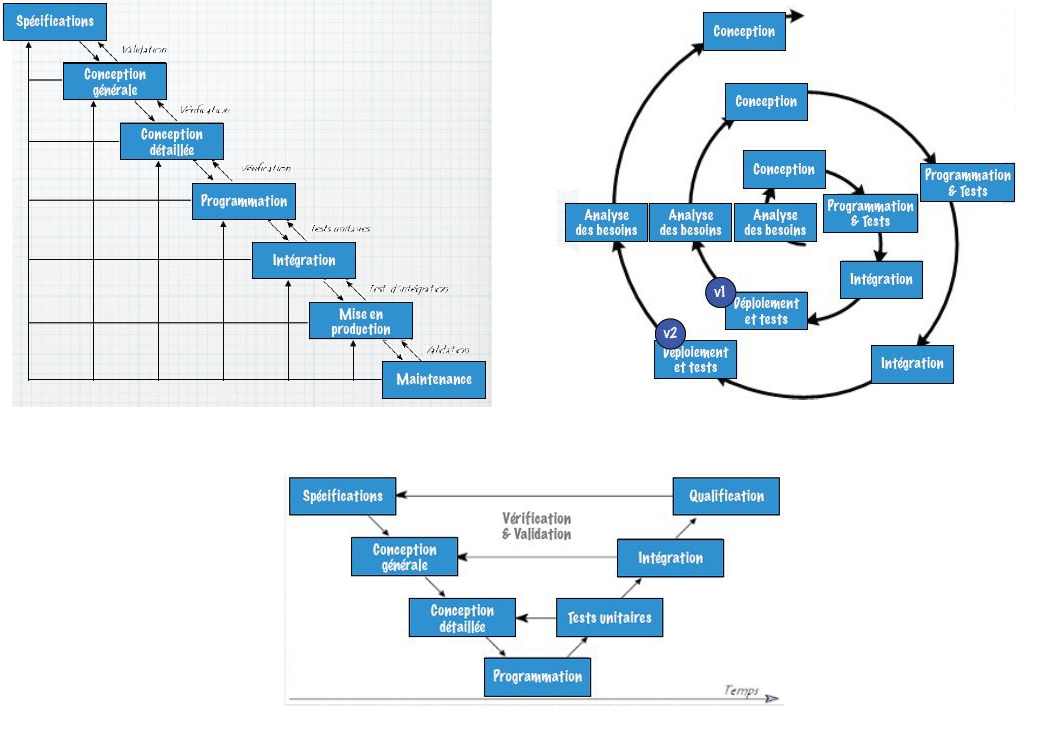
\includegraphics[scale=0.58]{processus_developpement_example.jpg}
  \caption{Différents processus de développement possibles}
  \label{processus_developpement_example}
\end{figure}

La figure~\ref{processus_developpement_example}
montre 3 exemples de processus de développement qui existent.

En haut à gauche, on retrouve le \textbf{modèle en cascade avec retour}.
Celui-ci tient compte du fait que l'on ne peut bâtir
un toit sans avoir les fondations.
Ainsi une fois l'étape une terminée,
on passe à la suivante et ainsi de suite en cascade.
Cependant un retour à l'une des phases précédentes est possible mais
la modification de celle-ci à un important coût sur le reste du développement,
ce qui rend cette approche peu pratique et non efficace.

Au milieu, on observe le \textbf{cycle en V}.
Il s'agit d'une amélioration du modèle précédant
car il permet de limiter le retour aux étapes précédentes.

A droite, le \textbf{modèle en spirale} reprend l'idée du cycle en V mais
recommence à chaque boucle tout le processus de manière à obtenir
des versions successives de plus en plus complètes.

Le meilleur modèle pour la conception orientée objet est
typiquement \textbf{itératif et incrémental}.
Ainsi la figure~\ref{processus_developpement_choisi}
illustre les différentes étapes de ce modèle.
On retrouve ainsi la phase d'INCEPTION où l'on
décrit l'objectif et l'ampleur du projet.
Ensuite, lors de l'ELABORATION, on imagine comment on va réaliser le système.
La phase de FABRICATION, décrite ci-dessous, est itérative et incrémental.
Pour finir la phase de TRANSITION permet d'optimiser le logiciel
en le testant et améliorant les performances.
\begin{figure}[h]
  \centering
  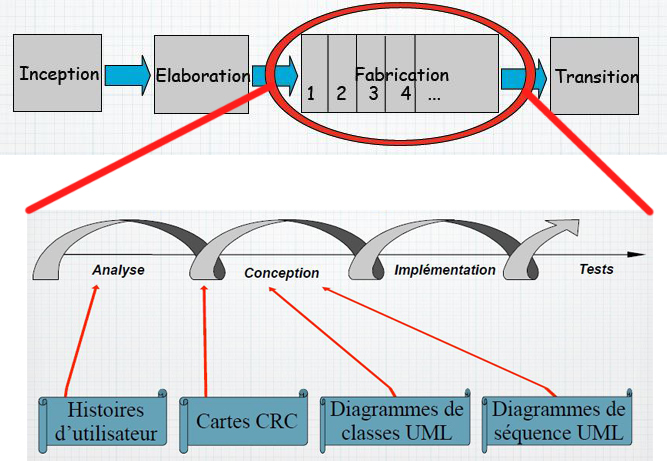
\includegraphics[scale=0.65]{processus_developpement_choisi.jpg}
  \caption{Processus itératif et incrémental choisi}
  \label{processus_developpement_choisi}
\end{figure}

La phase de FABRICATION reprend différentes itérations tels que
\begin{itemize}
  \item l'analyse par le biais d'histoires d'utilisateurs,
  \item la transition analyse-conception via les cartes CRC,
  \item la conception grâce aux diagrammes de classes UML et
  \item diagrammes de séquences UML
  \item pour arriver à l'implémentation.
\end{itemize}

\subsection{Les histoires utilisateur}
Dans un premier temps,
il faut définir ce qu'on appelle les
\textbf{histoires utilisateur} (user stories).
Celles-ci définissent les besoins,
les exigences de l'application.
On distinguera les besoins fonctionnels (fonctionnalités de l'application) et
les besoins non-fonctionnels (fiabilité, performance).
Généralement une histoire est une courte description d'un besoin
dans un langage de haut niveau compréhensible par tous.
Chaque histoire suit le schéma basique suivant :
\begin{quote}
  \emph{En tant que ``rôle'',
  \\je veux ``action'',
  \\afin d' ``atteindre un objectif''.}
\end{quote}
Il est important de ne pas trop détailler les histoires
et de les écrire à la voix active.
Aussi, pour le programmeur,
on peut ajouter le temps que l'on pense qu'il faudra pour
implémenter cette fonctionnalité à notre application.
Typiquement une histoire prend 2 jours à implémenter.
Voici deux exemples d'histoires utilisateurs :
\begin{itemize}
  \item \emph{En tant que} nouvel utilisateur de l'application,\\
    \emph{afin d'}adapter l'information fournie par l'application à mon âge,
    ma langue préférée et mes centres d'intérêts,\\
    \emph{je veux} pouvoir encoder un profil
    personnalisé lors du premier démarrage de l'application.
  \item	\emph{Afin de} pouvoir modifier mon profil personnalisé,\\
    \emph{en tant qu'}utilisateur connu par l'application,\\
    \emph{je veux} pouvoir changer mon profil personnalisé à n'importe
    quel moment via un menu dédié et,
    si mon utilisateur est actif,
    les informations fournies par l'application s'adapteront immédiatement
    à mon nouveau profil.
\end{itemize}

Le mot clé ``INVEST'' caractérise une bonne histoire utilisateur :
\begin{description}
  \item[Indépendant] Il faut rendre chaque histoire
    le plus indépendante les unes des autres.
  \item[Négociable] Une histoire n'est pas fixée une fois pour
    toute, la conversation avec le client peut amener à la modifier.
  \item[Valuable] Chaque histoire à
    sa propre valeur en fonction de son importance.
  \item[Estimable] À chaque histoire est associé un
    ``coût'' d'implémentation.
  \item[Small]Une histoire ne doit pas
    être trop grande (ni trop petite) sinon elle peut être divisée.
  \item[Testable]On peut tester si une histoire est réalisée ou pas.
\end{description}

\subsection{Les cartes CRC}
Les cartes CRC, pour \textbf{classes, responsabilités et collaborations},
permettent, comme leur nom l'indique,
d'obtenir une première idée des objets et classes qu'il faudra implémenter.
Ces classes auront certaines responsabilités en fonction des collaborations
qu'elles auront avec d'autres classes.

Propice pour le travaille en groupe,
cette méthode use de l'utilisation de petites cartes
permettant une représentation visuelle facile.
Chaque carte correspond à une classe,
contient une brève description de celle-ci,
ses responsabilités et collaborations (voir figure~\ref{carte_CRC}).

\begin{figure}[h]
  \centering
  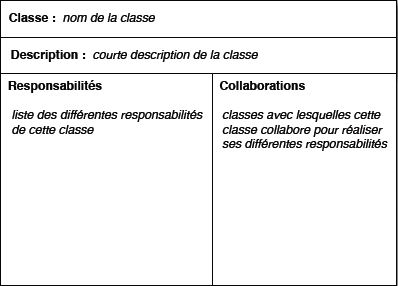
\includegraphics[scale=0.9]{carte_CRC.jpg}
  \caption{Modèle d'une carte CRC}
  \label{carte_CRC}
\end{figure}

Il est à noter que chaque classe possède au minimum une collaboration,
en effet si elle n'en avait pas elle ne servirait à rien.

\subsection{Le diagramme de classes UML}
La transformation des cartes CRC en
\textbf{diagramme de classes Unified Modeling Language} est assez simple.
Son but est d'exprimer de manière générale la \emph{structure statique}
d'un système en termes de classes et des relations entre elles.

Dans un tel diagramme (voir figure~\ref{diagramme_classes}),
les \emph{classes} sont représentées par des boîtes.
Une boîte a un nom qui décrit ce qu'elle est (et non ce qu'elle fait)
et contient généralement des attributs et des opérations applicables
aux instances de cette classe.
Pour les attributs,
ils ont généralement la syntaxe suivante:
visibilité \textbf{nom} : ``Type[multiplicité] = valeurInitiale''.
Seul le nom est obligatoire.
Les opérations ont la syntaxe suivante:
``visibilité \textbf{nom}(nomArg: Type=valeur,...) : Type''.
De même, uniquement le nom est obligatoire.

\begin{figure}[h]
  \centering
  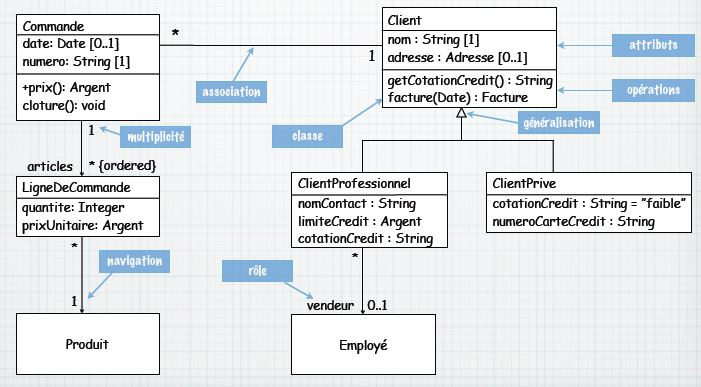
\includegraphics[scale=0.8]{diagramme_classes.jpg}
  \caption{Exemple d'un diagramme de classes UML}
  \label{diagramme_classes}
\end{figure}

\hspace*{-.75cm}Les différentes multiplicités possibles sont les suivantes :
\begin{description}
  \item[m] doit avoir exactement m (peut valoir *)
  \item[m..n] peut avoir entre m et n
  \item[m..*] minimum m
\end{description}
Les différents modes de visibilité sont les suivants :
\begin{description}
  \item[+]	Public, ouvert aux autres classes
  \item[\#]	Protégé, uniquement visible par les sous-classes
  \item[-]	Privé, uniquement accessible par cette classe
\end{description}
Des \textbf{contraintes} sur les attributs sont notés entre accolades.
Des \textbf{notes} peuvent être ajoutées au diagramme pour le clarifier.
Une note se manifeste par une boîte repliée qui est
reliée en pointillé à la boîte qu'elle clarifie.
On explicite aussi les \textbf{attributs dérivés} par la présence
d'un / avant le nom de l'attribut.
Un attribut est dérivé si sa valeur peut être retrouvée
grâce à d'autres attributs.
La figure~\ref{diagramme_classes_addon} illustre
comment représenter un attribut dérivé et sa contrainte dans une note associée.
\begin{figure}[h]
  \centering
  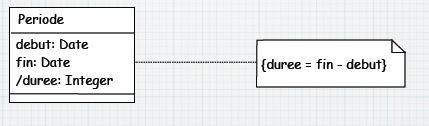
\includegraphics[scale=1]{diagramme_classes_addon.jpg}
  \caption{Représentation d'un attribut dérivé, d'une contrainte et d'une note}
  \label{diagramme_classes_addon}
\end{figure}

Pour exprimer une \textbf{association binaire},
on relie simplement les deux classes concernées.
On utilise en fait les associations lorsqu'un attribut n'est pas de type primitif.
Ainsi si on veut exprimer le fait qu'un client a des commandes (objet),
on le relie à la classe Commande.

Sur la ligne d'association,
on retrouve diverses informations tel qu'un nom (plus sens de lecture),
deux rôles (un a chaque extrémité) et les multiplicités associées aux classes.

Si l'association n'est pas à double sens
(c'est à dire si la classe A peut accéder à B mais pas l'inverse),
alors on placera une flèche (plutôt qu'une ligne) allant de A vers B.
On dit alors que c'est une \textbf{navigation}.

La figure~\ref{diagramme_classes_association}
représente une exemple d'association binaire.
\begin{figure}[h]
  \centering
  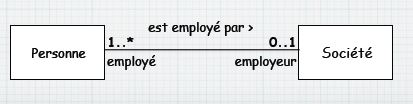
\includegraphics[scale=1]{diagramme_classes_association.jpg}
  \caption{Exemple d'une association binaire entre employé et employeur}
  \label{diagramme_classes_association}
\end{figure}

Une \textbf{généralisation} exprime que certaines classes
``dérivent'' d'une classe mère,
est une sorte de...
En java, on dit qu'une classe hérite d'une autre.
Cela se représente par une flèche ouverte.
Cela peut être nécessaire notamment dans le cas d'une
\textbf{classe abstraire} non instanciée mais qui
est présente pour clarifier les choses.
La figure~\ref{diagramme_classes_generalisation} représente ces deux concepts
\begin{figure}[h]
  \centering
  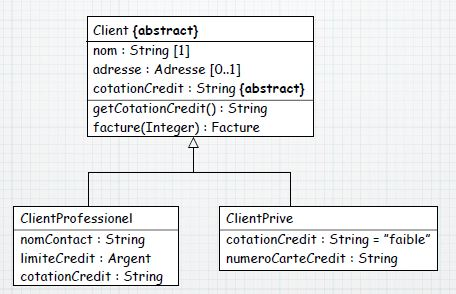
\includegraphics[scale=0.8]{diagramme_classes_generalisation}
  \caption{Exemple d'une généralisation et d'une classe abstraite}
  \label{diagramme_classes_generalisation}
\end{figure}

Il existe encore d'autres relations aux notations particulières.
Celles-ci sont reprises sur la figure~\ref{diagramme_classes_relations}.

On peut retrouver des \textbf{dépendances}.
Représenté par une flèche en pointillé,
elle est ornée d'un mot-clé qui décrit la relation
d'utilisation entre la source et la cible.
On distingue
\begin{description}
  \item[call]
    la classe source appelle une opération dans la classe cible,
  \item[create]
    la classe source crée une instance de la classe cible,
  \item[use]
    la classe source a besoin de la classe cible pour son implémentation.
\end{description}

\begin{figure}[h]
  \centering
  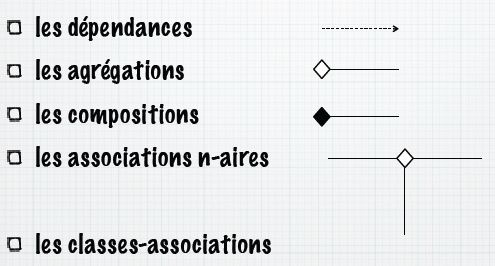
\includegraphics[scale=0.6]{diagramme_classes_relations}
  \caption{Notations des autres relations}
  \label{diagramme_classes_relations}
\end{figure}

L'\textbf{agrégation} représente une association non symétrique dans laquelle
une des extrémités joue un rôle prédominant par rapport à l'autre extrémité.
La différence avec l'association est floue et on ne l'utilisera donc pas.

La \textbf{composition} décrit une relation de contenance
physique (exemple : un polygone contient des points).

L'\textbf{association n-aire} relie plus de deux classes entre elles.
Généralement le lieu de rencontre peut être remplacé par une nouvelle
classe que l'on nomme \textbf{classe-association}.
Par exemple,
l'association Etudiant-Enseignant-Salle peut donné lieu à la classe Cours.

Lors de la réalisation d'un diagramme de classe UML,
il est important de pensé orienté objet,
et de bien penser à toutes les responsabilités,
opérations qu'une classe doit pouvoir effectuer.

\subsection{Le diagramme de séquence UML}
Dernière étape du processus de développement,
le \textbf{diagramme de séquence UML} permet de penser
la \emph{structure dynamique} de l'application.
Rappelons en effet que le diagramme de classes traitait
de la \emph{structure statique} de l'application.
Contrairement au diagramme de classes qui se basait sur les cartes CRC,
le diagramme de séquences se base sur les histoires
utilisateurs pour se structurer.
Typiquement, un diagramme de séquence décrit le comportement d'un
seul scénario et ne regroupera donc qu'une ou quelques histoires utilisateurs.
Sur l'axe horizontal,
on retrouvera les objets \emph{participants} et sur
l'axe vertical la chronologie des événements.
Un diagramme est constitué de \emph{messages} et
est toujours initialisé par un \emph{message trouvé}.
La figure~\ref{diagramme_sequences} montre un
exemple de diagramme avec ses différents composants.

\begin{figure}[h]
  \centering
  \hspace*{-0.25cm}
  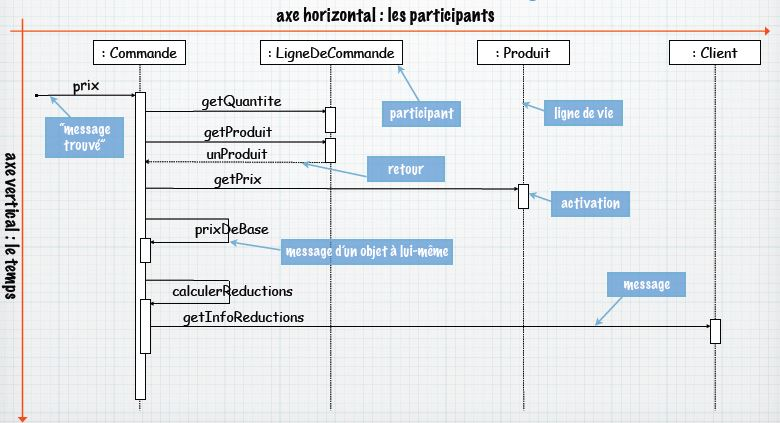
\includegraphics[scale=0.75]{diagramme_sequences.jpg}
  \caption{Composants d'un diagramme de séquences}
  \label{diagramme_sequences}
\end{figure}

Chaque participant est représenté par une ``boîte de ligne de vie''.
Une collection d'un type de participants sera représenté par une double boîte.
Des messages, représenté par des flèches,
partent de cette ligne de vie et ont la syntaxe suivante
\begin{verbatim}
retour = message(paramètre : typeParamètre) : typeRetour
\end{verbatim}
Le message est essentiel et les autres informations peuvent être omises.
Un message particulier est celui qui initiale le diagramme:
le message trouvé; il est représenté par un cercle noir.
Une ligne de vie possède une ou plusieurs barre d'activation
indiquant quand un participant est actif dans une interaction.
A un message correspond une réponse ou retour qui a la syntaxe:
\begin{verbatim}
valeurDeRetour = message(paramètre)
\end{verbatim}
Cette syntaxe fait deux choses en même temps : le message et le retour.
On peut expliciter les deux en faisant deux étapes:
le message comme décrit ci-dessus et le retour que l'on présentera
par une flèche en pointillé sur laquelle on écrit la valeur de retour.
Un objet peut également s'envoyer un message à lui-même.

Le diagramme de séquence permet aussi la création et la destruction d'objets.
La manière de procéder est illustré
par la figure~\ref{diagramme_sequences_objet}.
\begin{figure}[h]
  \centering
  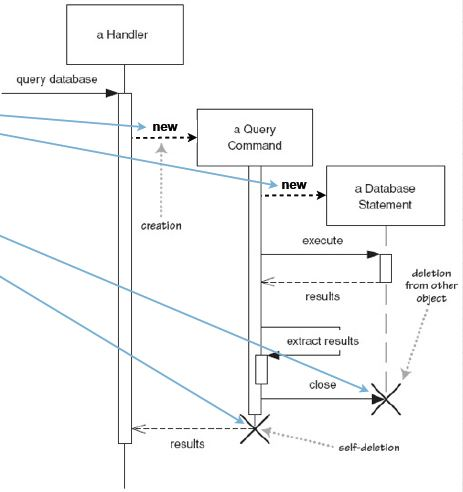
\includegraphics[scale=0.75]{diagramme_sequences_objet.jpg}
  \caption{Création et destruction d'objets dans un diagramme de séquences}
  \label{diagramme_sequences_objet}
\end{figure}

Pour terminer,
il faut pouvoir modéliser les structures conditionnelles et itératives.
Pour cela,
UML utilise des cadres (voir figure~\ref{diagramme_sequences_cadres}).
Un cadre est muni d'un \emph{opérateur} et d'une \emph{garde}.
\begin{figure}[h]
  \centering
  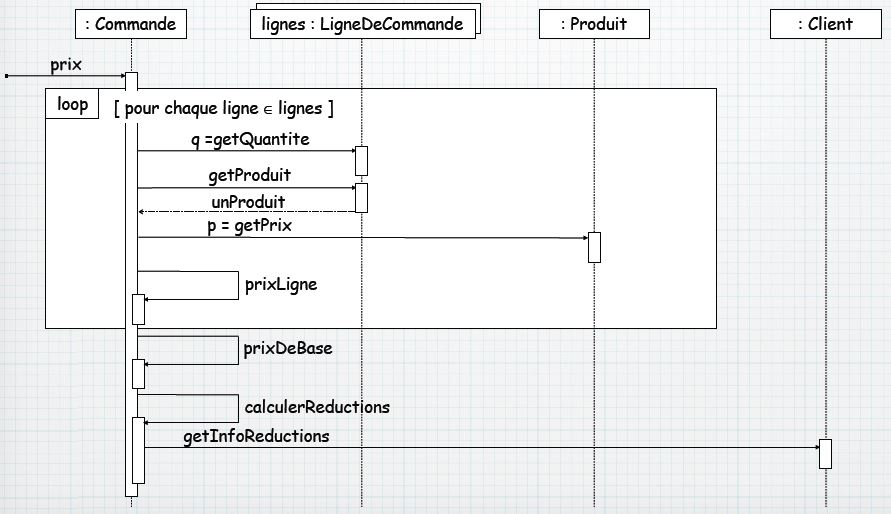
\includegraphics[scale=0.60]{diagramme_sequences_cadres.jpg}
  \caption{Exemple d'un cadre itératif dans un diagramme de séquence}
  \label{diagramme_sequences_cadres}
\end{figure}
Les trois opérateurs usuels sont les suivants
\begin{description}
  \item[alt] représente la condition if-else où le else est
    une garde séparé du if par des pointillé.
  \item[loop] représente la boucle for
  \item[opt] représente le condition if
\end{description}

\end{document}
